\chapter{A model for scintillating systems}

In this chapter a model for scintillating system is presented. 
The complex chain that leads from the interaction of a $\gamma$ quantum in a crystalline lattice is formalized in a statistical framework, in order to single out the contributions of the various processes that lead to resolution losses.

The aspects investigated involve the impact on time resolution of light yield (or photons collected), Cerenkov yield, rise and decay time for a multi-exponential scintillation pulse.
In order to do that we extended the model presented in \cite{Seifert2012}, to include Cerenkov photons produced by low energy $\gamma$ photons.
The role of Cerenkov processes is analysed with respect to analog time pick up techniques, which will be later used in this work. The role of rise time will be further discussed in the next chapters.

\section{Signal formation}

Rise time is the result of a complex chain of relaxation mechanisms of the electron hole pairs produced by the incoming ionizing radiation. The process is stochastic, and it is characterized by large statistical fluctuations at each step, thus determining a non-zero observed rise time, as shown in figure \ref{fig:chain}.
The relaxation steps have been summarized in \cite{Lecoq2014} as follows:
\begin{itemize}
\item 10$^{-16}$-10$^{-14}$ seconds: the incoming ionizing radiation creates deep holes in inner core bands and electrons in the conduction band. Secondary electronic excitation are successively created, via electron electron scattering and Auger processes
\item 10$^{-14}$-10$^{-12}$ seconds: below the electron-electron scattering threshold ($\sim$ 2E$_{g}$) the thermalization of electronic excitations starts. At this stage phonons are produced, leading electrons to the bottom of the conduction band and holes to the top of the valence band
\item 10$^{-12}$-10$^{-10}$ seconds: at this stage thermalized electrons and holes interact with defects and impurities in the lattice (formation of excitons, $V _{K}$ centres and self-trapped excitons). 
\item 10$^{-10}$-10$^{-8}$ seconds: finally radiative and/or non radiative recombination occurs.
\end{itemize}
\begin{figure}[htbp]
\begin{center}
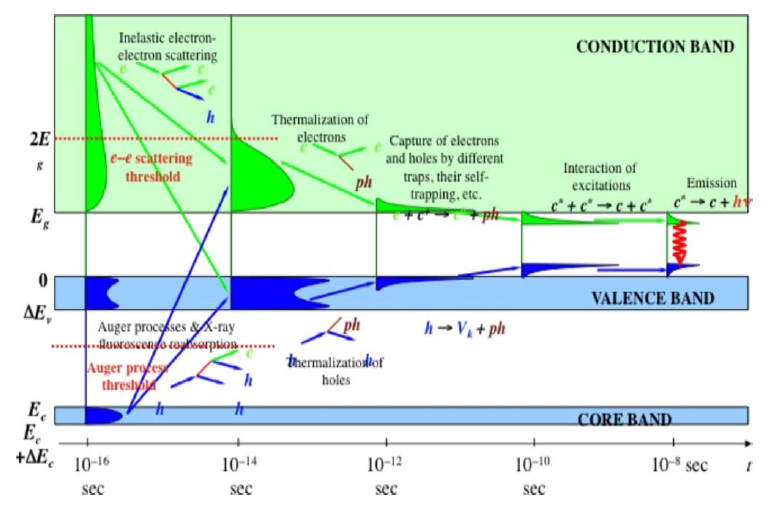
\includegraphics[width=14cm]{../Pictures/Chapter_4/chain.png}
\end{center}
\caption[Relaxation of electron and holes]{Relaxation scheme for incoming radiation with relative time scales of the processes involved \cite{Lecoq2014}.}
\label{fig:chain}
\end{figure}

Two additional processes should be considered. The production of Cerenkov photons may bring a non negligible amount of prompt photons in the first 50-100 ps of the rising signal.
Moreover the photons collected must be coupled out to the photo detector, so that at the end of the chain the signal collected is the convolution of different stochastic processes. Transportation stage will be dealt with mainly in chapters 5 and 6.

\subsection{Scintillation pulse}
It is typical to describe \cite{Hyman1963} the scintillation pulse as a sum of exponentials. The processes introduced in the previous paragraph, focus the attention on the last step of recombination, and the subsequent radiative transitions. 
All the processes that characterize electron hole relaxation and particularly thermalization of the pairs, lead to oscillations with respect to the start of the scintillation pulse determining a non zero rise time.
For all the practical purposes of this work rise time will be modelled by one or more exponential time components $\tau _{r}$. 
For what concerns recombination, the radiative transitions can be described by one ore more exponential decay times $\tau _{d}$.
In the case of LSO:Ce, for example, the transition takes place between the lowest 5d level, which lies just below the conduction band, and two 4f levels, above the valence band. The parity allowed transition accounts for very fast decay times ($\sim$ 40 ns).

We can consider, then, the absorption of a $\gamma$ photon at a time $\theta$. 
For many scintillators, we can describe the probability density function for the emission times as the convolution of two exponential functions representing the energy transfer processes and the radiative decay \cite{Shao2006}:
\begin{equation}
p_{t}(t|\theta) = \int _{-\infty}^{\infty} \exp{\left( -\frac{t'}{\tau _{r}}\right) } \exp{\left(-\frac{t-t'}{\tau _{d}}\right) } \theta (t') \theta (t-t') dt'
\end{equation}
In the case different processes contribute to the scintillation pulse via different energy transfer mechanisms, it may be necessary to consider them \cite{Seifert2012}
\begin{equation}
p _{t}(t|\theta) = \begin{cases} 0, & t < \theta \\ \sum _{i} S_{i} \frac{1}{\tau _{d, i} - \tau _{r, i}} \cdot \left[ \exp{\left( -\frac{t-\theta}{\tau _{d,i}}\right)} - \exp{\left( -\frac{t-\theta}{\tau _{r,i}}\right) } \right], & t > \theta \end{cases}
\end{equation}
where S$_{i}$ is the intensity of the fluorescent component and the sum goes over the components.

\subsection{Cerenkov pulse}
As shown in chapter 3, a non negligible amount of Cerenkov photons can be produced by a low energy $\gamma$ event. 
In particular this has an impact in the extraction of a time stamp for a certain event, since we often make use of single threshold crossing. In fact we mainly rely on the information carried by a single photon. Thus if the number of Cerenkov photons is bigger than zero, photons collected at the very beginning of the pulse can come with a high probability from a Cerenkov event.

In order to define a Cerenkov pulse, the Geant4 software was used. The software package will be fully analysed in the next chapter. For the sake of simplicity, we consider the time of production of Cerenkov photons that follow a $\gamma$ photo electric interaction in a LSO crystal. The delay is given by the geometry of the experiment, in this case the main interest lies in the width of the distribution.
\begin{figure}[htbp]
\begin{center}
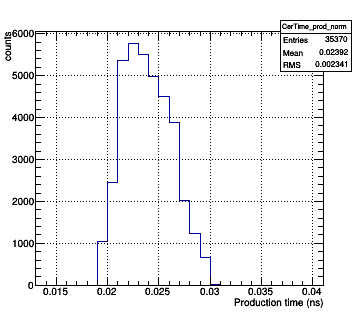
\includegraphics[width=9cm]{../Pictures/Chapter_4/cerenkov_time.png}
\end{center}
\caption[Cerenkov production]{Cerenkov production profile in LSO by a 511 KeV photon simulated with the Geant4 software package.}
\label{fig:cer_see}
\end{figure}
In this chapter no transit time variation for the photons is considered, so that the distribution of Cerenkov photons modelled is the production distribution, shown in \ref{fig:cer_see}. 
For most practical purposes, and considering that the time scale of the physical quantity, we can safely consider the Cerenkov pulse as a Gaussian curve in time, with a spread in production time of $\sigma =$ 3 ps.
It is important to underline that, while the scintillation yield of a certain crystalline species will depend strongly on the growing method (doping concentration, type of dopant, etc.), the Cerenkov yield depends essentially on density and index of refraction. This means that the respective intensity of the two photon production phenomena should be scaled accordingly. In this study we relied on scintillation values measured in laboratory (see chapter 6 and following for the measurement setup) and Cerenkov values extracted from Geant4 simulations.

\section{The Cramer-Rao lower bound}
In general, the emission times t of the detected N photons can be considered statistically independent and identically distributed (iid).
Most photo detectors can be modelled as ideal photon counters, able to detect a time stamp for every incoming photon, a set $T_{N} = \{ t_{1}, t_{2}, ..., t_{N}|\theta \}$.

In order to account for the smearing introduced by the resolution of the detector on the photon time stamps, it is necessary to define its response $p_{T}$. In particular  it can be modelled by a Gaussian with a variance equal to the single photon time resolution (SPTR) and a mean equal to the transit time $t_{tr}$. The function is truncated at $t=0$ not to allow negative transit times.
\begin{equation}
p_{T} = \frac{1}{\sqrt {2\pi} \sigma _{sptr}} \exp{\left[-\frac{-(t-t_{tt})^{2}}{2(\sigma _{sptr})^{2}}\right]}
\end{equation}
The corresponding pdf for the time stamps is then a convolution of the photon emission rate and the smearing of the detector.
\begin{equation}
p_{t_{n}}(t|\theta) = p_{t}(t|\theta)\ast p_{T}(t)= \int _{-\infty}^{\infty}p_{t}(t-x|\theta) \cdot p_{T}(x)dx = \int _{0}^{t-\theta}p_{t}(t-x|\theta) \cdot p_{T}(x)dx
\end{equation}
And the integral gives
\begin{equation}
\begin{align*}
p_{t_{n}}(t|\theta) &= A \cdot \sum _{i} \frac{S_{i}}{\tau _{d,i} - \tau _{r,i}} \cdot \left[ a_{\tau _{d, i}}(t|\theta) - a_{\tau _{r,i}}(t|\theta)\right]\\
& + B \cdot \exp{\left( -\frac{(t_{tr} + \mu _{cer} - t)^{2}}{2(\sigma _{cer}^{2}+ \sigma _{sptr}^{2})} \right)}\\
& \cdot \left[ erf\left( \frac{-t_{tr}\sigma _{cer}^{2} + \mu _{cer} \sigma _{sptr}^{2} -t\sigma _{sptr} ^{2} +(t-\mu _{cer})(\sigma _{cer}^{2}+\sigma _{sptr}^{2})}{\sqrt{2}\sigma _{sptr}\sigma_{cer}\sqrt{\sigma _{sptr}^{2}+\sigma_{cer}^{2}}} \right)\right.\\
& \left. - erf \left( \frac{-t_{tr}\sigma _{cer}^{2} + \mu _{cer} \sigma _{sptr}^{2} -t\sigma _{sptr} ^{2}}{\sqrt{2}\sigma _{sptr}\sigma_{cer}\sqrt{\sigma _{sptr}^{2}+\sigma_{cer}^{2}}} \right)\right]
\end{align*}
\end{equation}
where 
\begin{equation}
\begin{align*}
a _{\tau}(t|\theta) &= \frac{1}{2} \exp{\left(\frac{\sigma _{sptr} ^{2} - 2t\tau +2\theta \tau + 2t_{tr}\tau}{2\tau ^{2}}\right)} \\
& \cdot \left[ erf\left( \frac{t-\theta -t_{tr} - \frac{\sigma ^{2}_{sptr}}{\tau}}{\sigma _{sptr}\sqrt{2}} \right) + erf \left( \frac{t_{tr}+\frac{\sigma ^{2} _{sptr}}{\tau}}{\sigma _{sptr}\sqrt{2}} \right)
\end{align*}
\end{equation}
$A$ is the normalization for the scintillation curve, B is the normalization for the Cerenkov curve, $\sigma _{cer}$ is the spread of Cerenkov production and $\mu _{cer}$ is the mean of Cerenkov production, that will be considered at $\theta$ (we assume that the scintillation pulse and the Cerenkov pulse start at the same moment).
The bi exponential model used is shown in figure \ref{fig:models}, as well as the modification in the rise time induced by Cerenkov photons and detector smearing.
\begin{figure}[htbp]
\begin{center}
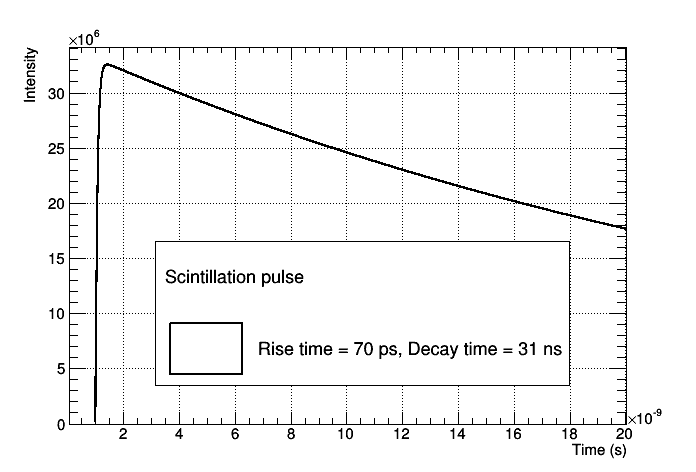
\includegraphics[width=8cm]{../Pictures/Chapter_4/scint_new.png}
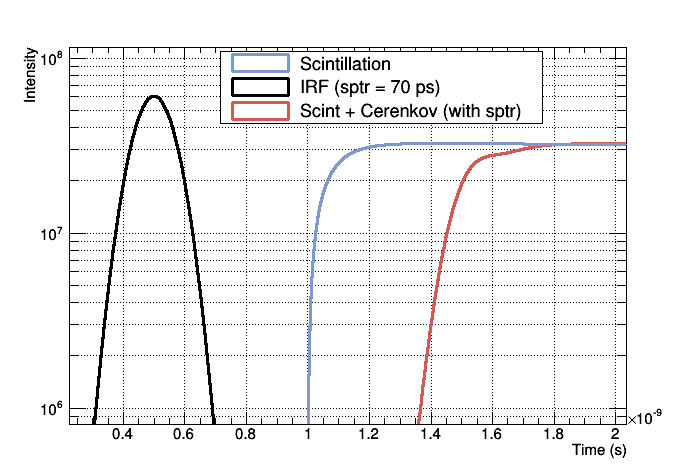
\includegraphics[width=8cm]{../Pictures/Chapter_4/tot_new.png}
\end{center}
\caption[Model functions]{Bi exponential model used (left) and modification on the rise introduced by Cerenkov photons and detector smearing (right)}
\label{fig:models}
\end{figure}

The Fisher Information $I(\theta)$ is defined as
\begin{equation}
I(\theta) = \int _{-\infty} ^{\infty} \left[ \frac{\partial}{\partial \theta} \ln p_{t_{n}}(t|\theta) \right] ^{2} p_{t_{n}}(t|\theta)dt
\end{equation}
Since the samples are iid, the information is additive, so that
\begin{equation}
I(\theta) = N \cdot \int _{-\infty} ^{\infty} \left[ \frac{\partial}{\partial \theta} p_{t_{n}}(t|\theta) \right] ^{2} \frac{1}{p_{t_{n}}(t|\theta)}dt
\end{equation}
The Cramer Rao theorem states that the variance of any unbiased estimator $\hat{\theta}$ of $\theta$ is bounded by the reciprocal of the Fisher information:
\begin{equation}
var(\hat{\theta})\geq \frac{1}{I(\theta)}
\end{equation}
In a PET-like experiment the interest lies in the estimate of the photon time of interaction $\theta$.
Statistically speaking the Cramer Rao theorem gives the intrinsic time resolution limit for any given scintillator with defined fluorescent parameters.


\section{The order statistics}
If a specific order in the set of recorder timestamps is assumed, it is evident that they are neither independent nor identically distributed. By sorting the elements in $T_{N}$ we can create an ordered set $T_{\bar{N}} = \{ t_{\bar{1}} \leq t_{\bar{2}} \leq ... \leq t_{\bar{N}} \}$. The pdf for the nth-order statistics is given by \cite{Seifert2012}
\begin{equation}
f_{n|N} (t|\theta) = \binom{N}{n} \cdot n \cdot P_{t_{n}}^{n-1}(t|\theta) \cdot \left[ 1-P_{t_{n}}(t|\theta) \right] ^{N-n}\cdot p_{t_{n}} (t|\theta)
\end{equation}
In this case the set is not iid; thus considering an estimator using a unique time stamps, as the case of analog SiPMs, the Fisher information is
\begin{equation}
I_{n}(\theta) = \int _{-\infty} ^{\infty} \left[ \frac{\partial}{\partial \theta} \ln f_{n}(t|\theta) \right] ^{2} f_{n}(t|\theta)dt
\end{equation}
   
\section{Intrinsic time resolution}

We can now use the framework expanded in the previous section to infer the timing properties of a simplified setup characterized by five parameters:
\begin{itemize}
\item the light yield
\item the Cerenkov yield
\item the rise time
\item the decay time
\item the time spread in Cerenkov emission 
\end{itemize}
Thanks to the Cramer-Rao theorem it is possible to extract the lower bound in coincidence time resolution for a setup with specified parameters. This means that the entire set is used in the statistics, regardless of the method used to extract the time information: this represents a theoretical value given the information contained in the set.
It is important to stress that for the moment we do not consider any spread introduced by the transport of photons inside the volume. This will be considered in the next chapter, where Monte-Carlo simulations will allow to introduce this additional parameter.

In order to weight the importance of the various model parameters in the calculation of the time resolution of the system, we first make use of the entire statistical set, that is we find the lower bound.
In a first moment the Cerenkov yield is set to zero.
This is the case for crystals with very low collection efficiency or very low Cerenkov production. In the case of samples used in this study this number can be estimated to range between 2 and 10 depending on the crystal and the wrapping condition. 

The first consequence of assuming iid samples is that the information is proportional to the number of photons collected.
This implies inverse proportionality for the lower limit on the variance. If we assume 5000 photo electrons produced by a LSO crystal coupled to a standard photodetector at 511 KeV, we can focus on the time dependence of the model.

A complete treatment for the Cramer Rao lower bound dependence on scintillation photons is presented in \cite{Gundacker2014}. The rise time is an important parameter to accurately estimate the CTR. A shown in \cite{Gundi}, a change from 20 ps to 110 ps in rise time, entails a CTR variation of 20 FWHM. This can be seen from figure \ref{fig:cramer_rise}. A careful analysis suggest that the scintillation rise time has is comparable to SPTR when considering their impact on CTR. This can be seen by comparing the plots for rise time and SPTR variation shown in figure \ref{fig:cramer_rise}.

\begin{figure}[htbp]
\begin{center}
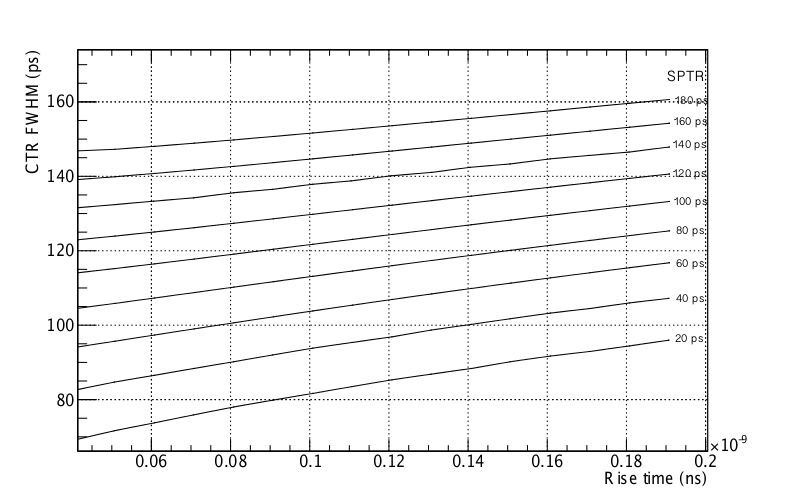
\includegraphics[width=10cm]{../Pictures/Chapter_4/rise_CTR.png}
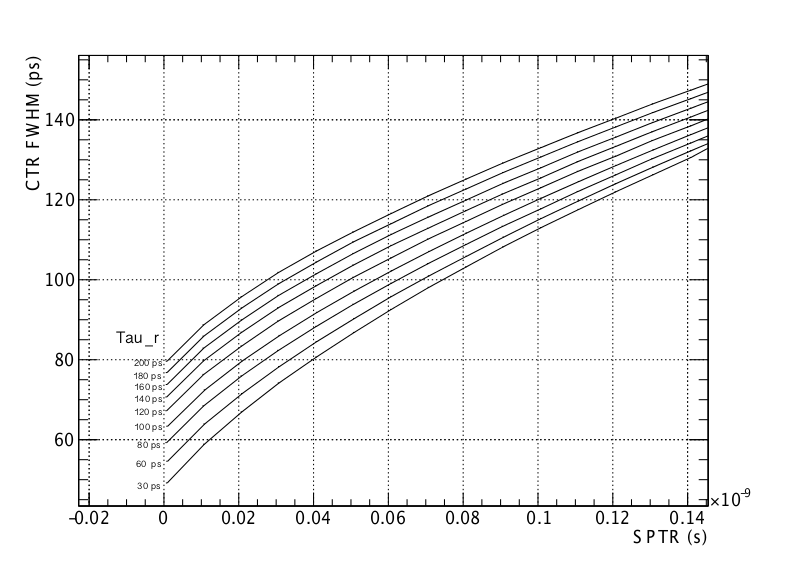
\includegraphics[width=10cm]{../Pictures/Chapter_4/sigma_CTR.png}
\end{center}
\caption[Cramer Rao evolution - rise time]{Cramer Rao lower bound as a function of rise time for different values of SPTR (left) and as a function of SPTR for different values of rise time (right)}
\label{fig:cramer_rise}
\end{figure}
%In figure \ref{fig:} and \ref{fig:} is shown the dependance of the CTR from the time profiles of the crystals,
%and the SPTR.
%Imrp

The role of Cerenkov photons becomes somehow more obscure in this situation. As shown in figure \ref{fig:cramer_cer}, a small number of Cerenkov photons collected can in principle worsen the lower bound achievable. This is due to the fact that the fast emission can introduce a higher variance when combined to the bi exponential statistics. This is strongly correlated with the light yield of the crystal measured, since this effect is more and more pronounced as the light yield grows. Indeed when the light yield of the crystal is low, we start relying mainly on Cerenkov photons, whose number depends only on the optical characteristics of the medium. As the RMS of the Cerenkov collection is lower, if we could collect a significant number of photons we could in principle achieve better coincidence time resolutions.
%This simply states that a device which could make use of Cerenkov photons in significative number would reach a better value for time resolution since it would not depend on the time profile of the scintillation.
% that is from rise time and decay time. The SPTR value is set to 70 ps, which is a value consistent to the SiPMs used in this work and can deliver the top performance in terms of time resolution.
%The decay time is shown to influence the time resolution more importantly. Indeed decreasing the decay time 
\begin{figure}[htbp]
\begin{center}
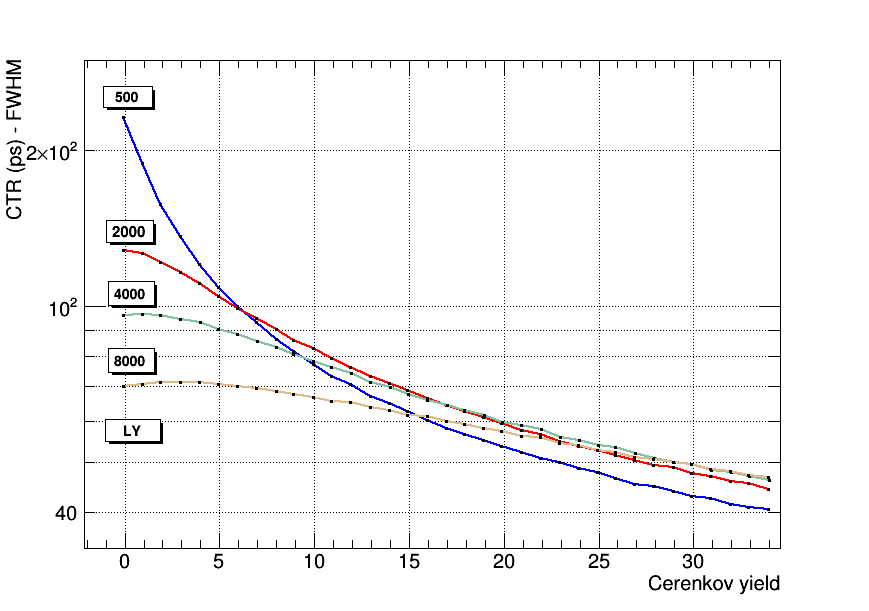
\includegraphics[width=10cm]{../Pictures/Chapter_4/CY_LY_cramer_rao.png}
%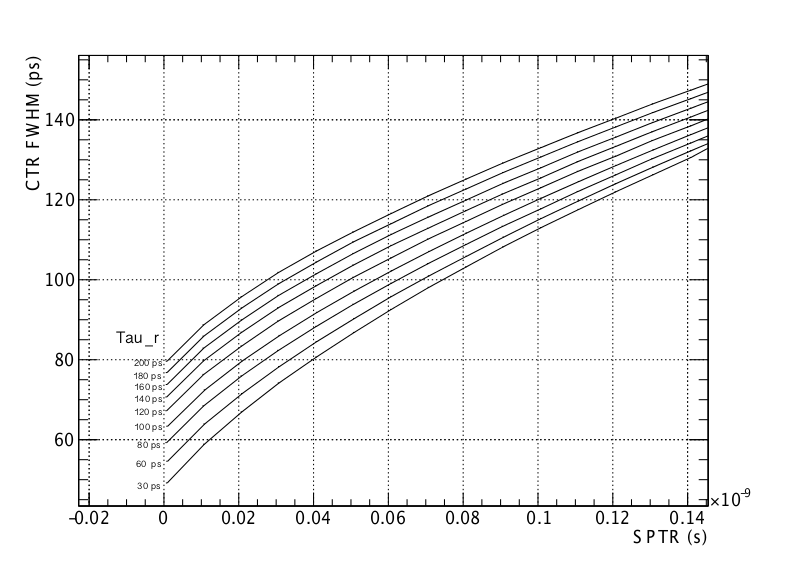
\includegraphics[width=6cm]{../Pictures/Chapter_4/sigma_CTR.png}
\end{center}
\caption[Cramer Rao evolution - Cerenkov]{Cramer Rao lower bound as a function of Cerenkov photons collected for different scintillation light output values}
\label{fig:cramer_cer}
\end{figure}

\section{Effects on signal extraction}

If we consider a time pick up system similar to the one used in this study, it is necessary to extend the analysis to the variance associated to specific photon ranks. 
This is the case of SiPMs used in PET detectors, as shown in \ref{fig:crossing}, as the signal is a build up of single cells firing. We then basically rely on the information of a threshold crossing. An example of this time pick up method will be shown in chapter 8.
The threshold crossing is associated with a certain number of photons piling up. Therefore the specific variance associated to the rank of the photon over the threshold determines the resolution achievable. This resolution is higher than the Cramer Rao lower bound, which is obtained considering the entire set of information brought by the photon statistics.
\begin{figure}[htbp]
\begin{center}
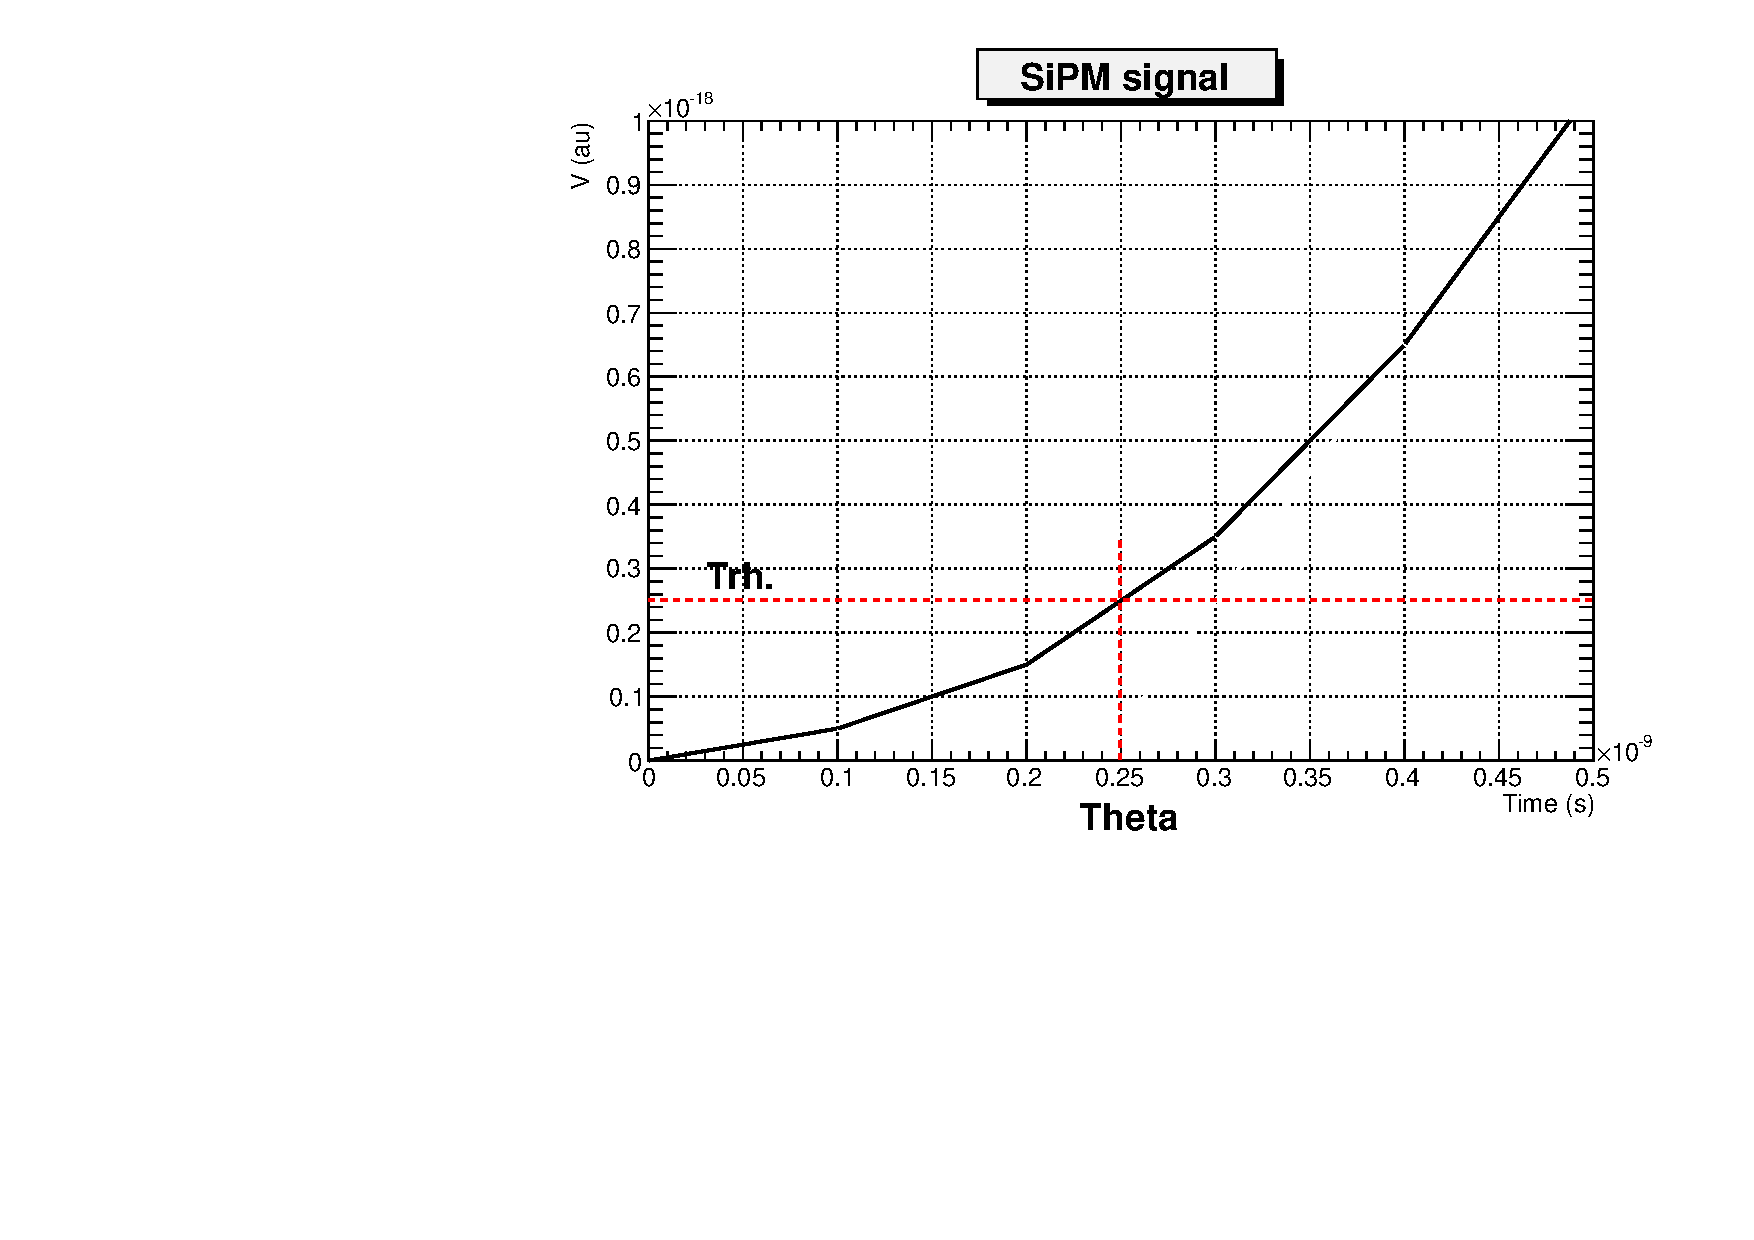
\includegraphics[width=10cm]{../Pictures/Chapter_4/crossing.pdf}
\end{center}
\caption[Threshold crossing example]{Example of a time pickup method based on threshold crossing. Theta is the time stamp extracted, the curve is a rising edge of a SiPM, modelled as a sequence of slopes. It is the method used by the NINO chip used in this work.}
\label{fig:crossing}
\end{figure}
In figure \ref{fig:rank} the time distribution for photon of different rank following the order statistics previously obtained is shown, for the case with SPTR = 0 and SPTR = 70 ps.
\begin{figure}[htbp]
\begin{center}
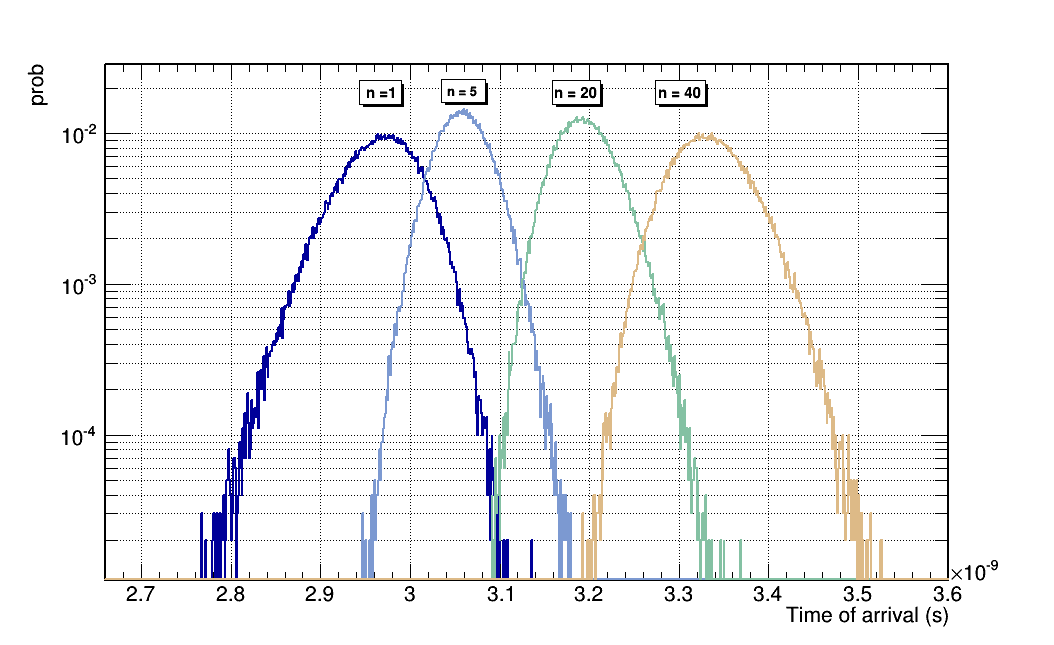
\includegraphics[width=10cm]{../Pictures/Chapter_4/photon_rank.png}
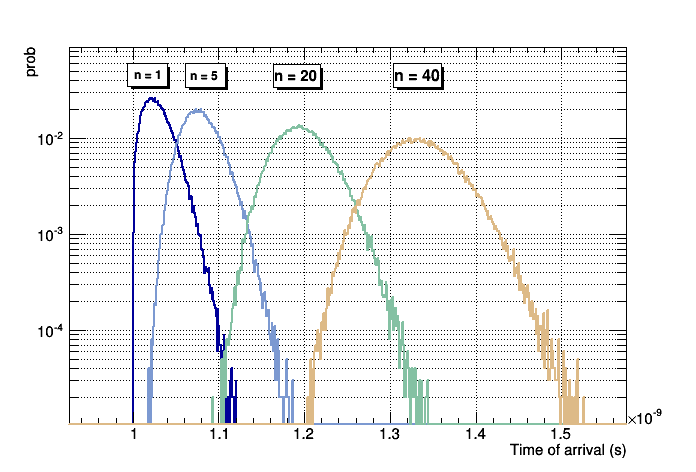
\includegraphics[width=10cm]{../Pictures/Chapter_4/photon_rank_no_smear.png}
\end{center}
\caption[Photon rank RMS]{Time distribution for photon of different rank without (left) and with (right) detector smearing}
\label{fig:rank}
\end{figure}
It is already clear that, in general, it is not the first order statistics that provides the estimation with the lower variance. This is due to the smearing introduced by the detector. Indeed, a non-smeared time profile would entail a monotonous increase of the variance, as shown in figure \ref{fig:rise_rank}, where the variance of the n-th photon collected is plotted, at different rise time values.
In the same plot we focus on the role of rise time on the shape of the curve in the case of non zero SPTR. 
Indeed a faster rise time is associated not only with lower variances for photons of the same rank, as expected, but it changes the order statistics with the smallest variance.
\begin{figure}[htbp]
\begin{center}
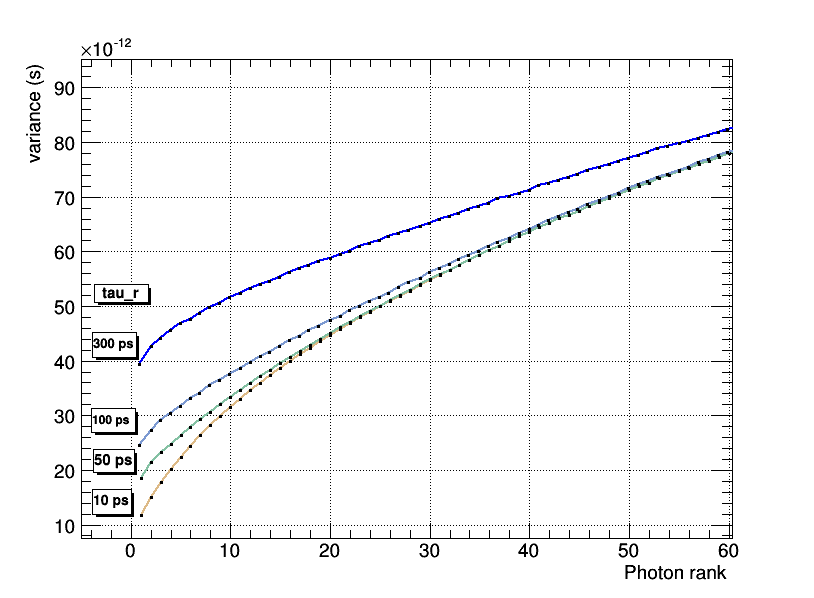
\includegraphics[width=10cm]{../Pictures/Chapter_4/taur_rank_nosptr.png}
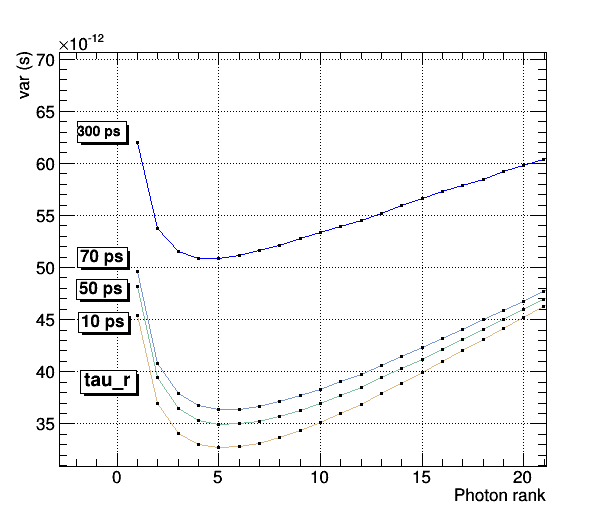
\includegraphics[width=10cm]{../Pictures/Chapter_4/tau_r_rank.png}
\end{center}
\caption[Rank variance - rise time]{The evolution of the variance of the n-th rank photon for different rise time values with SPTR = 0 (left) and SPTR = 70 (right).}
\label{fig:rise_rank}
\end{figure}
As can be seen from a comparison of the variance curves for photons of different ranks and lower bounds for the same parameters, a detector which makes use of a single time stamp can not reach the lower bound. Thus the late photons adds small information to the statistics. An approach to include this photons in the analysis could make use of digital pick up techniques. 

For what concerns Cerenkov photons, it is shown in figure \ref{fig:rise_rank} that they have a significant impact only if at least five of them can be collected. Indeed for a very small number of Cerenkov photons the CTR resolution is the same, and so the variance associated with the order statistics with the smallest variance.
Things change when a higher number of Cerenkov photons are collected. In this case the ratio between scintillation photons and Cerenkov photons can be quite small, so that we start to rely mainly on the latter.
This can be the case for crystal such as LuAG or PbWO$_{4}$. As will be shown in the next chapter, for our purposes the Cerenkov pulse will introduce a modified rise time with respect to the absolute value.
\begin{figure}[htbp]
\begin{center}
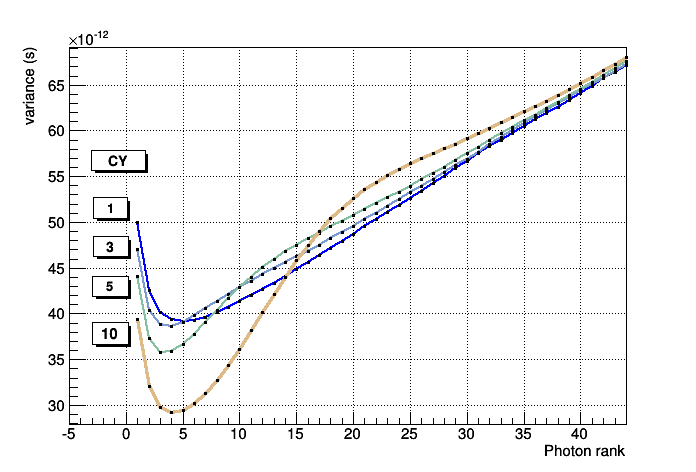
\includegraphics[width=10cm]{../Pictures/Chapter_4/CER_photon_rank.png}
\end{center}
\caption[Rank variance - Cerenkov]{The evolution of the variance of the n-th rank photon for different Cerenkov yields.}
\label{fig:rise_rank}
\end{figure}

